\documentclass[11pt]{article}

\usepackage[T1]{fontenc}
\usepackage{lmodern}
\usepackage{amsmath,amssymb}
\usepackage{booktabs}
\usepackage{array}
\usepackage{graphicx}
\usepackage{float}
\usepackage{longtable}
\usepackage[margin=1in]{geometry}
\usepackage{xurl}
\usepackage[hidelinks]{hyperref}
\hypersetup{
  pdftitle={Source-Locked Evaluation of Black-Box QUBO and Ising Heuristics: Public Evidence from Gset Max-Cut and BiqMac Certified-Value Checks},
  pdfauthor={Bernardo De Araujo Coutinho Mendonca},
  pdfsubject={Black-box QUBO and Ising solver evaluation protocol},
  pdfkeywords={QUBO, Ising, Max-Cut, evaluation, source lock, reproducibility}
}
\usepackage{authblk}
\usepackage[numbers,sort&compress]{natbib}

\newcolumntype{L}[1]{>{\raggedright\arraybackslash}p{#1}}
\makeatletter
\setlength{\@fptop}{0pt}
\makeatother

\title{Source-Locked Evaluation of Black-Box QUBO and Ising Heuristics: Public Evidence from Gset Max-Cut and BiqMac Certified-Value Checks}
\author[1]{Bernardo De Araujo Coutinho Mendonca}
\affil[1]{Independent Researcher, United States of America\\
\texttt{acmbernie@gmail.com}}
\date{}

\begin{document}
\maketitle

\begin{abstract}
This paper presents a source-locked, append-only evaluation protocol for proprietary black-box QUBO and Ising solvers and applies it to B1Brain across five locally controlled compute tiers. Such solvers are difficult to compare when benchmark instances, objective conventions, baseline values, failed runs, and timing measurements are not reported consistently. The public 2026-05-31 evidence snapshot contains 20,223 completed solver rows across public-safe non-overlapping evidence lanes, including a complete 15,807-row redacted G72/G77/G81 Gset Max-Cut frontier extract. The protocol contributes public source identifiers, checksum manifests for released artifacts, claim-pin discipline with an impossible-result guard, non-claim row accounting, lane-level row reconciliation, and tail-distribution reporting over large seed volumes. On G72, G77, and G81, B1Brain reaches best gaps of 2.455\%--2.654\% to current best-known heuristic values. In the BiqMac parity lane, certified-value rows correspond to \texttt{proven\_optimum} values from the official BiqMac library and are used to test impossible-result handling rather than to claim broad BiqMac dominance. A three-row equal-$N=30$ controlled-baseline summary is retained only as a context and release-boundary artifact because raw baseline rows and command pins are not public. The paper makes no speed, throughput, energy-efficiency, statistical-significance, fairness, public baseline-rerunability, or proof-of-optimum statement. The contribution is an auditable public evidence package for black-box optimization claims, not a claim of Max-Cut leadership.
\end{abstract}

\section{Introduction}
QUBO and Ising formulations provide a common language for combinatorial optimization problems such as routing, scheduling, allocation, and selection. A growing solver ecosystem targets these formulations, including classical heuristics, GPU-accelerated emulators, quantum annealers, digital annealers, and hybrid systems. As the ecosystem expands, the central challenge is not only building solvers but credibly comparing them.

Three failure modes recur in optimization benchmarking. First, baseline ambiguity can conflate proven optima, best-known heuristic values, and undocumented values. Second, measurement conflation can compress solution quality, wall-clock time, and energy use into a single headline. Third, selective reporting can hide capability boundaries, dependency failures, or launcher errors. This paper treats the evaluation process itself as the contribution.

We evaluate B1Brain as a black box. Its implementation is outside the scope of this paper; all claims are based on externally observable inputs, outputs, and execution records. This boundary is deliberate. It supports independent review without exposing protected implementation details and makes the methodology applicable to other proprietary or open QUBO/Ising solvers.
Although B1Brain is the case study, the protocol is solver-agnostic: the same source-lock, append-only row accounting, exclusion, and checksum checks could be applied to open-source heuristics, hardware emulators, annealers, or other proprietary optimizers.

The paper contributes:
\begin{enumerate}
  \item a source-locked baseline protocol with citation, source-identifier, and released-artifact integrity pinning;
  \item a claim-pin protocol with impossible-result detection for certified-value datasets;
  \item append-only result accounting that separates claim-valid rows from non-claim rows;
  \item tail-distribution reporting over large seed volumes; and
  \item a local-control protocol for offline-capable execution across heterogeneous compute tiers.
\end{enumerate}

\paragraph{Scope of claims.}
This paper claims evidence-integrity discipline, repeated local execution, and bounded quality distributions on disclosed benchmark lanes. It does not claim proven optimality, global Max-Cut leadership, timing superiority, energy efficiency, public rerunability of controlled baselines, or full public reproducibility of solver internals. Where solution bitstrings, unredacted JSONL records, or controlled baseline command details would strengthen independent reproduction, they are identified as controlled-review artifacts requiring separate public-release and IP review.

\paragraph{Evidence snapshot.}
The campaign is substantial. The final evidence matrix records completed execution across five hardware tiers: entry/mobile GPU, two prosumer GPUs, one dedicated local RTX5090 workstation tier, and a unified-memory tier. The frontier Max-Cut lane contains 15,807 completed claim-valid rows across Tier2, Tier3, and Tier4; within that lane, Tier4 contributes 9,300 completed rows from the dedicated RTX5090 queue. Tier1 and Tier5 add entry-tier and structure/stress evidence. These counts do not establish quality leadership by themselves; they establish repeated successful execution, robustness, and auditability.

\section{Related Work}
The Max-Cut problem has a long optimization literature, including semidefinite-programming approximation baselines \cite{goemans1995maxcut}. The Gset Max-Cut suite remains a standard benchmark for Ising and QUBO solvers. Recent work by Zick reports new best-known values for G72, G77, and G81 and describes those values as appearing optimal, not as independently proven optima \cite{zick2025}. Khan and Shukla report a new best-known G63 value, illustrating that the Gset frontier is still active \cite{khan2025g63}. Comparative benchmarking work has studied Ising-machine performance on Max-Cut at scale \cite{shaglel2025maxcut}, while practical Ising-machine benchmarking emphasizes fair accounting for problem mapping, constraints, and consumed compute time \cite{ohno2024qkp}. Reviews of Ising hardware emphasize time-to-solution and success-probability measurement rather than claims of universal asymptotic advantage \cite{mohseni2022ising}. Simulated Bifurcation was introduced as a Hamiltonian-dynamics heuristic for combinatorial optimization \cite{goto2019sb}; the small open SB summary retained in this paper uses a specific cited open implementation \cite{openSB}, not Toshiba's commercial Simulated Bifurcation Machine or all SB-family solvers. MQLib provides a published heuristic-library reference point for Max-Cut and QUBO comparisons \cite{dunning2018mqlib}. MaxCut-Bench highlights the importance of standardized Max-Cut instances and traditional local-search baselines such as Tabu Search when comparing heuristic solvers \cite{nath2024maxcutbench}; this release does not include a public source-locked Tabu Search lane because that lane requires a pinned implementation or wrapper, exact restart policy, objective convention, stopping rule, and command record before it can be compared under the same source-lock standard.

Our work is positioned in this evaluation-methodology tradition. It does not disclose a new algorithm. It instead defines a source-locked, append-only, black-box measurement protocol and applies it to a locally controlled solver.

\paragraph{Positioning against comparable papers.}
This paper should be read differently from papers that announce a new best-known cut value or a new solver mechanism. Unlike frontier-value papers, it does not claim a new best-known Gset objective. Unlike broad public benchmark suites, it does not claim universal solver leadership. Its narrower contribution is to show how a proprietary black-box solver can be evaluated with source-locked baselines, public-safe summaries, explicit exclusion rules, cross-tier local execution, and distributional rather than cherry-picked reporting.

\section{Evaluation Methodology}
\subsection{Source-Locked Baselines}
Every external comparison value is tied to a source identifier, public citation, date, value type, and verification status. For G72, G77, and G81 we use the current best-known heuristic values reported by Zick: 7008, 9940, and 14060 respectively \cite{zick2025}. These values are treated as current best-known heuristic values. They are not treated as proven optima.

Benchmark instance identity is locked through public source references, instance names, objective conventions, and value-type labels before comparison. In the public source package, released result CSVs, summary tables, verifier scripts, and supplement artifacts are cryptographically checksummed; the standard public Gset instance files themselves are referenced by source and instance name, but are not redistributed or separately hashed in this release. This distinction prevents the public package from overstating independent instance-file digest verification while still binding reported objectives to disclosed benchmark identities and cited best-known values.

Source-locking also applies to comparison systems. The current public package pins the cited baseline sources and reports the controlled-baseline material as a context-only summary lane; exact baseline command lines, seed lists, compile options, and raw controlled rows remain a release gate before this lane should be treated as independently rerunnable.

\subsection{Claim Pins and Impossible-Result Detection}
Each result row carries a claim-pin status. A row can support a performance statement only when the run completed successfully and the input, objective convention, and baseline mapping pass validation. For datasets with externally certified objective values, any result exceeding the certified value is rejected as a data-integrity failure instead of being converted into a favorable gap.

The public BiqMac parity lane provides a concrete check of this guard. Across 90 released certified-value rows, zero rows exceed their source-locked certified reference value and 75 rows match that value exactly. This supports the integrity rule; it is not a broad BiqMac performance or dominance claim.

\subsection{Append-Only Records and Non-Claim Rows}
Results are written append-only. Failed attempts are preserved and categorized rather than overwritten. Rows with status values such as capability boundary, dependency failure, launcher error, or investigation failure are excluded from performance claims and accounted for separately. Row count alone is not sufficient; a valid performance denominator requires completed solver rows.

\subsection{Tail-Distribution Reporting}
Heuristic solvers can vary by seed or initialization. For each tier and instance, we report best, mean, standard deviation, P50, P90, and P95 gaps over claim-valid rows. Large seed volume is useful because it exposes robustness and tail behavior; it is not used to imply a fair matched-budget win against smaller-seed baselines. Because this paper excludes timing claims, tail distributions are used as a quality-stability audit, not as a time-to-solution or success-probability substitute.

The public extracts expose seed identifiers and append order for audit. They should be interpreted as released completed-run sequences with partially overlapping seed ranges across tiers, not as a paired-seed equivalence experiment and not as proof of independent random sampling beyond the recorded seed policy; raw queue-generation metadata remains a controlled-review artifact.

\subsection{Local-Control and Hardware Evidence Protocol}
The evaluation runs on locally controlled, offline-capable hardware tiers. In this paper, local execution control means the ability to execute and audit the solver on hardware under the evaluator's control without depending on a remote optimization service. The distinction from ordinary offline benchmarking is the audit requirement: a row is not admitted because a local job was launched, but because process liveness, expected hardware/runtime, source-locked input identity, completed-row status, and claim-pin checks all align. It is not a claim of security certification, lower cost, timing advantage, or energy efficiency. For active queues, three independent signals are required before claims are admitted: worker liveness, expected hardware and runtime presence, and recent completed JSONL result rows. Timing and throughput claims require dedicated, uncontended hosts and are excluded from this paper unless explicitly identified as dedicated timing evidence.

\section{Compute Campaign and Evidence Volume}
The central empirical point of this paper is that the solver was not evaluated through a small demonstration. It was exercised through a multi-day, append-only compute campaign with thousands of completed runs, cross-tier repeats, explicit row admissibility rules, and post-run exclusion checks.

\begin{table}[tbp]
\centering
\caption{Evidence-lane map and claim boundaries.}
\label{tab:lanemap}
\footnotesize
\begin{tabular}{@{}L{0.16\linewidth}L{0.17\linewidth}L{0.31\linewidth}L{0.28\linewidth}@{}}
\toprule
Lane & Public rows & Supports & Does not support \\
\midrule
Frontier quality & 15,807 per-run rows & G72/G77/G81 quality distributions and distribution-level cross-tier repeatability & Optimality, speed, energy, paired-seed equivalence, or global Max-Cut leadership \\
Gset breadth & 330 per-run rows & Broader Gset source-lock and execution breadth & Frontier-value leadership across all Gset instances \\
BiqMac parity & 90 per-run rows & Source-repaired certified-value parity checks & Broad BiqMac dominance \\
Controlled-baseline context & 3 summary rows & Release-boundary example for equal-$N$ summary reporting & Public rerunability, matched compute budget, statistical significance, or a solver-superiority claim \\
Tier1 entry & 126 authoritative rows & Entry-tier feasibility and decomposition-floor evidence & Performance superiority \\
Tier5 structure & 3,870 authoritative rows & Unified-memory structure and stress evidence & Gset frontier-performance claims \\
Deferred source-lock lanes & 0 public claim rows & G63/G64, Tabu Search/MaxCut-Bench, broader Gset and vertical follow-up scope & Current performance, leadership, timing, or rerunability claims \\
\bottomrule
\end{tabular}
\end{table}

\begin{table}[tbp]
\centering
\caption{Row-accounting reconciliation for commonly cited counts.}
\label{tab:rowaccounting}
\small
\begin{tabular}{@{}L{0.35\linewidth}rL{0.42\linewidth}@{}}
\toprule
Quantity & Count & Relationship to claims \\
\midrule
Final non-overlapping evidence lanes & 20,223 & Total completed solver rows across public-safe final lanes. \\
G72/G77/G81 frontier-quality lane & 15,807 & Primary distributional quality lane used in Table~\ref{tab:frontier}. \\
Tier4 RTX5090 frontier subset & 9,300 & Included inside the 15,807 frontier rows; not additive. \\
Gset breadth lane & 330 & Broader source-lock and execution breadth evidence. \\
BiqMac parity lane & 90 & Source-repaired certified-value parity subset. \\
Tier1 entry lane & 126 & Entry-tier feasibility plus repeat spot-check rows. \\
Tier5 structure lane & 3,870 & Unified-memory structure and stress evidence; not a Gset frontier lane. \\
Controlled-baseline context & 3 summary rows & Context only; not counted inside the 20,223 completed public-safe solver rows and not independently rerunnable from public files. \\
\bottomrule
\end{tabular}
\end{table}

\begin{figure}[H]
\centering
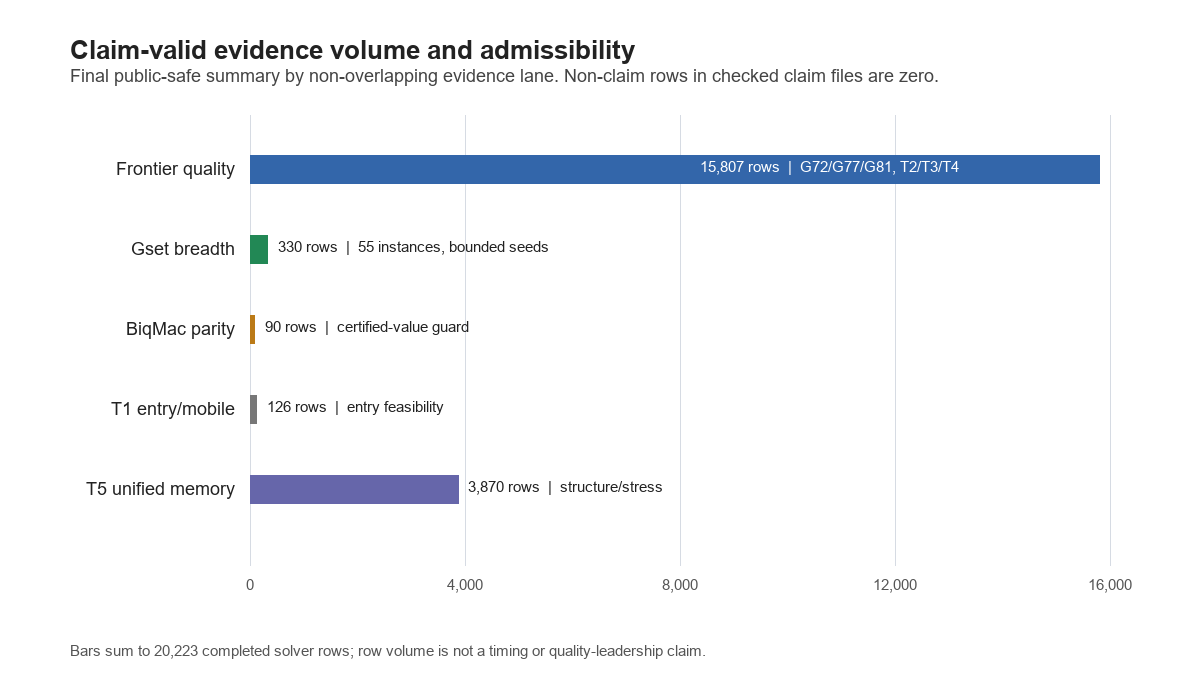
\includegraphics[width=0.92\linewidth]{figures/fig_evidence_volume_academic.png}
\caption{Claim-valid evidence volume and admissibility. Public-safe completed-row counts are reported by evidence lane; row volume supports repeated execution and auditability, not a timing or quality-leadership claim.}
\label{fig:evidencevolume}
\end{figure}

\begin{figure}[H]
\centering
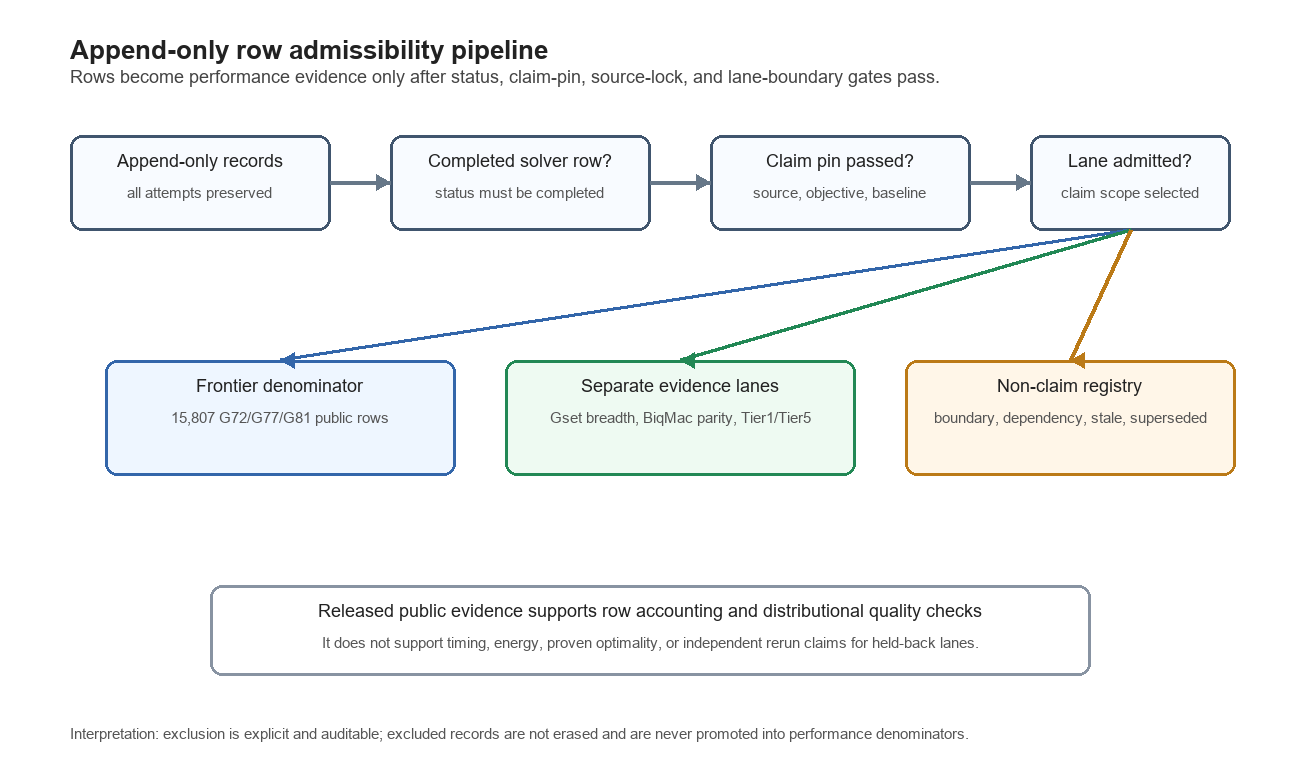
\includegraphics[width=0.96\linewidth]{figures/fig_row_admissibility_flow_academic.png}
\caption{Append-only row admissibility pipeline. Rows become performance evidence only after completed status, claim-pin validation, source-lock checks, and lane-boundary selection; excluded categories remain auditable outside performance denominators.}
\label{fig:admissibility}
\end{figure}

\noindent Figures~\ref{fig:evidencevolume} and~\ref{fig:admissibility} summarize the public evidence volume and the row-admissibility boundary. The evidence volume matters for two reasons. First, a heuristic solver should be judged by its distribution, not by one lucky seed. Second, a local-control claim is weak unless the same workload family runs on different local machines with independent runtime and row-integrity checks. This campaign supplies both kinds of evidence. Invalid, boundary, duplicate, stale, and dependency-failure records are retained outside the performance denominator rather than erased.

\section{Experimental Setup}
\subsection{Benchmark Instances}
The public-safe frontier results in this release focus on Gset instances G72, G77, and G81 because those instances have clean source-locked current best-known heuristic values and a complete public per-run frontier extract. They are structurally related large Gset Max-Cut instances and therefore form a narrow frontier lane, not a representative sample of every graph family. They are not the full benchmark campaign. Gset breadth and BiqMac parity lanes use bounded seed counts for coverage and integrity checks; the frontier lane is deep-sampled because it is the main distributional stability target. G63, G64, and other active Gset instances are excluded from the public frontier claim lane because this release does not yet provide final source-lock metadata and release artifacts for them. Tabu Search and MaxCut-Bench-style local-search baselines are likewise deferred until a reproducible public wrapper, random-restart policy, stopping rule, version pin, and command record are source-locked.

The public supplement separates broader evidence into distinct lanes: Gset breadth rows, source-repaired BiqMac certified-value checks \cite{biqmac}, synthetic structure-aware correctness tests, and held-back real-world-derived demonstrations. Here, source-repaired means that rows are admitted only after the public instance/reference-value mapping, objective convention, and certified-value association are corrected and verified against the cited source; no solver output is altered by this repair step. Unrepaired or mismatched rows remain outside performance claims. Those additional tracks support breadth, parity, and local-control evidence, but they are not used to claim frontier Max-Cut leadership.

\subsection{Hardware Matrix}
Table~\ref{tab:hardware} summarizes the local hardware evidence lane. Tiers are reported by class and externally relevant runtime properties, not by protected execution details.

\begin{table}[tbp]
\centering
\caption{Local hardware evidence matrix.}
\label{tab:hardware}
\small
\begin{tabular}{llll}
\toprule
Tier & Class & Accelerator & Claim-valid evidence \\
\midrule
1 & entry/mobile & GTX 1050 Ti & 120/120 completed; 6/6 repeat spot-check \\
2 & prosumer & RTX 4070 & 3,006 completed frontier rows; timing excluded \\
3 & prosumer & RTX 4060 Ti & 3,501 completed frontier rows \\
4 & dedicated workstation & RTX 5090 & 9,300 completed frontier rows \\
5 & unified-memory & APU / unified memory & 3,870 completed structure/stress rows \\
\bottomrule
\end{tabular}
\end{table}

\subsection{Controlled Baseline Context}
A small controlled-baseline summary records B1Brain alongside a specific cited open Simulated Bifurcation implementation \cite{openSB} and MQLib \cite{dunning2018mqlib}. It uses equal restart count ($N=30$) on the dedicated RTX5090 workstation tier. Equal $N$ matches the number of restarts only; it does not normalize per-restart work, wall-clock time, implementation efficiency, hardware utilization, or total computational budget. Because the public package does not release raw baseline rows, exact command pins, solver versions, build flags, seed lists, stopping rules, tuning policy, or distributional baseline traces, this lane is retained as context and as an example of claim-boundary discipline. It is not used as a public rerunability, fairness, statistical-significance, or solver-superiority claim.

\begin{table}[tbp]
\centering
\caption{Controlled-baseline context and current release boundary.}
\label{tab:baselineprotocol}
\footnotesize
\begin{tabular}{@{}L{0.15\linewidth}L{0.15\linewidth}L{0.18\linewidth}L{0.18\linewidth}L{0.18\linewidth}@{}}
\toprule
System & Public source & Controlled rows & Budget status & Public rerun status \\
\midrule
B1Brain & black-box solver & $N=30$ summary values & equal restart count; timing and compute-budget normalization excluded & executable and raw rows not public \\
Open SB implementation & cited open implementation & $N=30$ summary values & equal restart count; timing and compute-budget normalization excluded & command pins and raw rows not public \\
MQLib & published heuristic library & $N=30$ summary values & equal restart count; timing and compute-budget normalization excluded & command pins and raw rows not public \\
\bottomrule
\end{tabular}
\end{table}

The $N=30$ cap is intentional: it prevents the large-seed B1Brain robustness lane from being confused with a baseline contest that used thousands of B1Brain restarts. The summary values are shown in Appendix~\ref{sec:controlledappendix} to document what was checked and, more importantly, what is not claimed. Because distributional baseline traces and command records are not public, this table does not meet the same distributional or rerunability standard applied to B1Brain's public frontier extract. Stronger statistical, fairness, or rerun claims require releasing the controlled raw rows, exact baseline commands, and distributional baseline traces after separate clearance.

\section{Results}
\subsection{What the Campaign Shows}
The strongest supported claims are operational and methodological: source-locked comparisons, completed append-only rows across heterogeneous hardware, tight frontier gap bands over thousands of seeds, and honest exclusion of invalid rows. The evidence supports a repeatable local black-box optimization system under the disclosed protocol. It does not support Max-Cut quality leadership, and the paper does not claim it. This is a useful stress test for the protocol: the evidence framework does not flatter B1Brain, because it preserves deferred baseline artifacts and other cases where stronger validation is still missing.

\subsection{Large-Seed Frontier Robustness}
Table~\ref{tab:frontier} reports the final large-seed distribution for G72, G77, and G81 across Tier2, Tier3, and Tier4. These rows are claim-valid completed rows only. They support robustness and reproducibility claims, not direct matched-budget superiority claims.

\begin{scriptsize}
\begin{longtable}{@{}llrrrrrrrr@{}}
\caption{Large-seed frontier distribution: gap to current best-known heuristic value. T2/T3/T4 denote the RTX4070, RTX4060 Ti, and RTX5090 tiers.}\label{tab:frontier}\\
\toprule
Tier & Inst. & N & Obj. & Best & Mean & Std & P50 & P90 & P95 \\
\midrule
\endfirsthead
\toprule
Tier & Inst. & N & Obj. & Best & Mean & Std & P50 & P90 & P95 \\
\midrule
\endhead
T2 & G72 & 1006 & 6828 & 2.568\% & 3.166\% & 0.176\% & 3.168\% & 3.396\% & 3.453\% \\
T2 & G77 & 1000 & 9694 & 2.475\% & 3.065\% & 0.216\% & 3.038\% & 3.340\% & 3.422\% \\
T2 & G81 & 1000 & 13702 & 2.546\% & 3.132\% & 0.201\% & 3.115\% & 3.400\% & 3.471\% \\
T3 & G72 & 1167 & 6822 & 2.654\% & 3.167\% & 0.171\% & 3.168\% & 3.396\% & 3.453\% \\
T3 & G77 & 1167 & 9696 & 2.455\% & 3.077\% & 0.218\% & 3.058\% & 3.360\% & 3.441\% \\
T3 & G81 & 1167 & 13692 & 2.617\% & 3.133\% & 0.202\% & 3.129\% & 3.391\% & 3.471\% \\
T4 & G72 & 3100 & 6828 & 2.568\% & 3.167\% & 0.173\% & 3.168\% & 3.396\% & 3.453\% \\
T4 & G77 & 3100 & 9690 & 2.515\% & 3.086\% & 0.212\% & 3.078\% & 3.360\% & 3.441\% \\
T4 & G81 & 3100 & 13700 & 2.560\% & 3.149\% & 0.202\% & 3.144\% & 3.414\% & 3.499\% \\
\bottomrule
\end{longtable}
\end{scriptsize}

\clearpage

\subsection{Distribution Shape and Cross-Tier Diagnostics}
The public extract allows a reader to inspect the full gap distribution rather than only the printed summary statistics. Figure~\ref{fig:gapboxplot} summarizes median, interquartile, and 5th--95th percentile behavior by instance and tier, while Figure~\ref{fig:gapecdf} plots empirical CDFs from the same rows. The curves and box summaries are close across tiers, supporting the interpretation that the frontier lane is a distribution-level repeatability and quality-stability artifact rather than a single-machine result.

The cross-tier claim is deliberately distributional. The released frontier lanes use partially overlapping completed seed ranges across tiers, so Table~\ref{tab:tierstats} should be read as evidence that the public B1Brain frontier quality distribution is stable across the RTX4070, RTX4060 Ti, and RTX5090 runtime lanes. It is not a claim that every seed is paired across all hardware tiers or that identical seeds produce bit-identical trajectories across GPU architectures.

\begin{figure}[tbp]
\centering
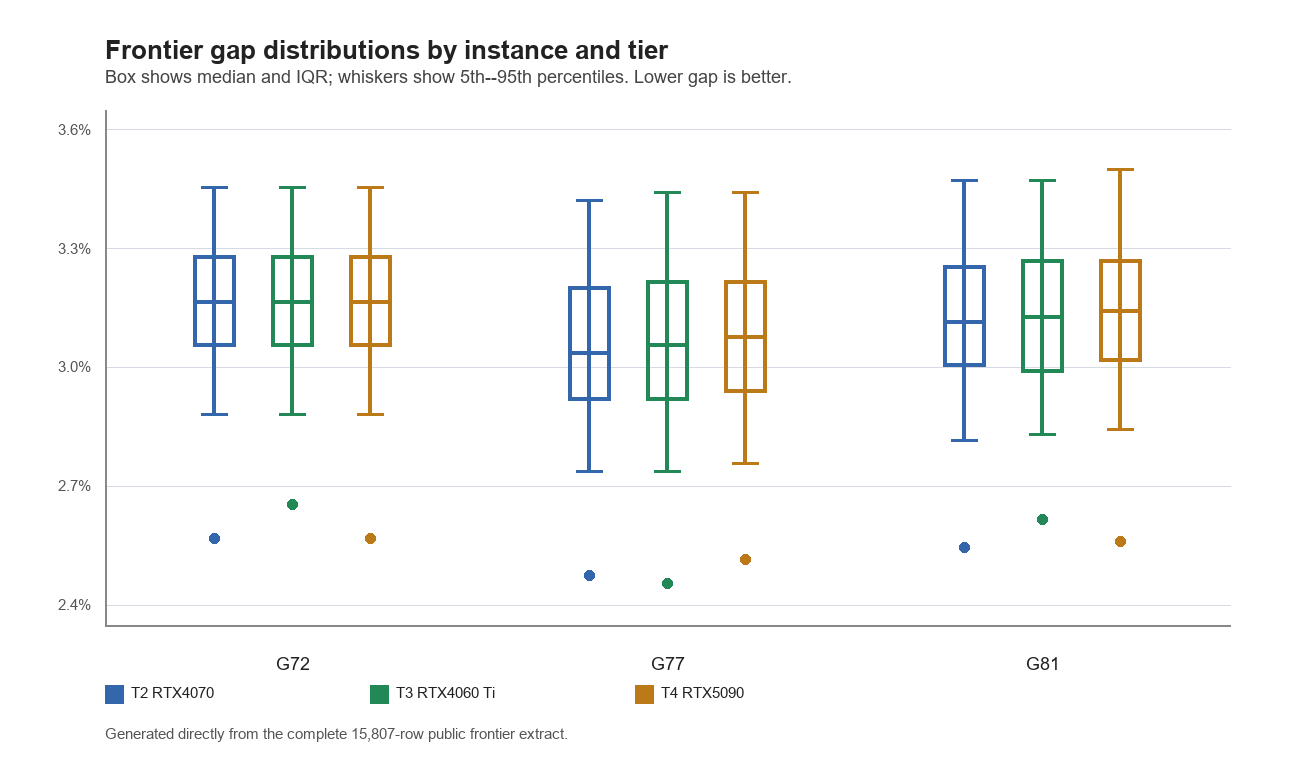
\includegraphics[width=0.96\linewidth]{figures/fig_gap_boxplot_academic.png}
\caption{Frontier gap distributions by instance and tier from the complete 15,807-row public frontier extract. Boxes show medians and interquartile ranges; whiskers show 5th--95th percentiles. Lower gap is better.}
\label{fig:gapboxplot}
\end{figure}

\begin{figure}[tbp]
\centering
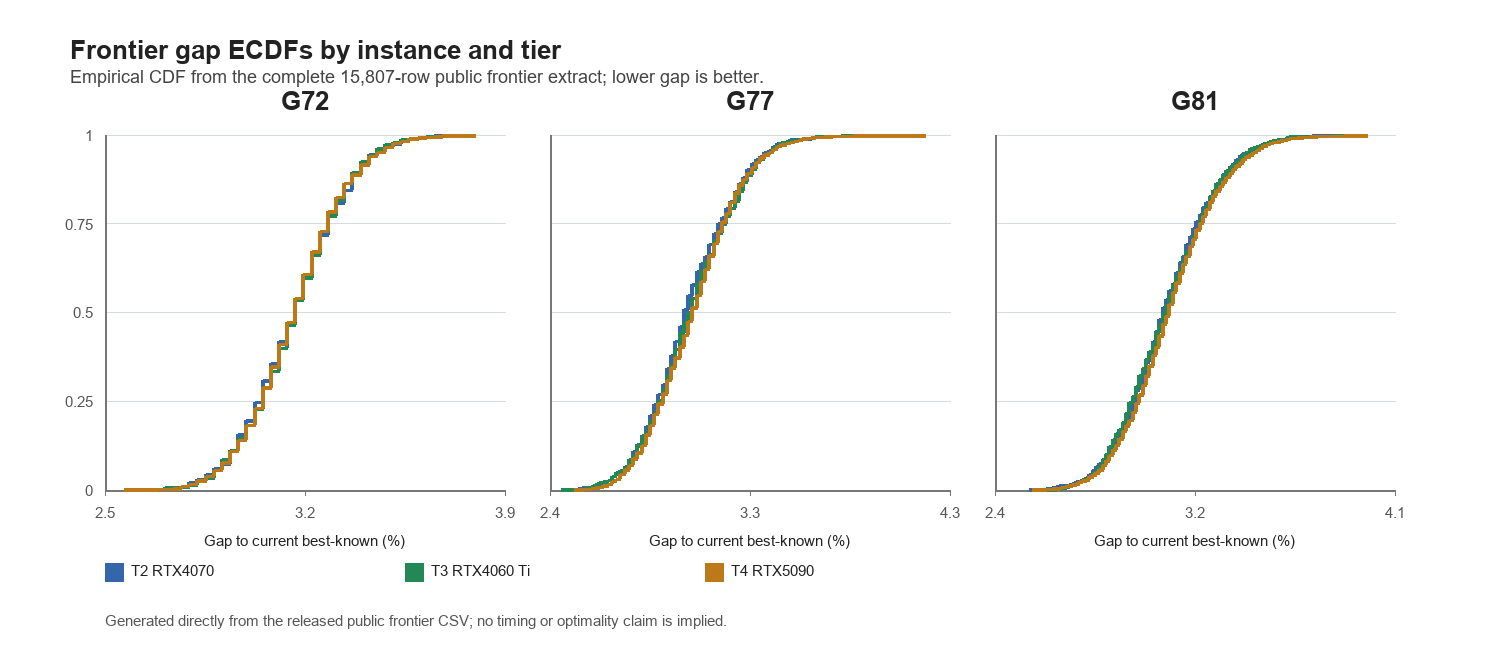
\includegraphics[width=0.96\linewidth]{figures/fig_gap_ecdf_academic.png}
\caption{Empirical CDFs of gap-to-best-known values from the complete 15,807-row public frontier extract. These plots make the tail-distribution claim visually inspectable from the released CSV; lower gap is better.}
\label{fig:gapecdf}
\end{figure}

\begin{table}[H]
\centering
\caption{Cross-tier distribution diagnostics from the public frontier extract. KS tests are descriptive diagnostics only; because the row counts are large, small absolute mean shifts below 0.03 percentage points can produce low p-values.}
\label{tab:tierstats}
\footnotesize
\begin{tabular}{llrrrr}
\toprule
Instance & Pair & $N_L$ & $N_R$ & Mean-gap delta & KS p-value \\
\midrule
G72 & T2 vs. T4 & 1006 & 3100 & 0.0008 pp & 0.942 \\
G72 & T3 vs. T4 & 1167 & 3100 & 0.0007 pp & 0.999 \\
G77 & T2 vs. T4 & 1000 & 3100 & 0.0208 pp & $5.35{\times}10^{-4}$ \\
G77 & T3 vs. T4 & 1167 & 3100 & 0.0087 pp & 0.140 \\
G81 & T2 vs. T4 & 1000 & 3100 & 0.0169 pp & 0.065 \\
G81 & T3 vs. T4 & 1167 & 3100 & 0.0159 pp & 0.010 \\
\bottomrule
\end{tabular}
\end{table}

All absolute mean-gap deltas in Table~\ref{tab:tierstats} are below 0.03 percentage points. Low $p$-values in this large-$N$ setting are therefore interpreted as distributional diagnostics rather than practically meaningful quality separations.

\clearpage

\subsection{Seed-Budget Plateau Diagnostic}
Large seed volume is most useful when it reveals the shape of solver behavior rather than simply increasing the row count. Figure~\ref{fig:seedplateau} plots the best gap observed so far within the Tier4 public frontier extract, ordered by public append sequence. The plateau indicates that the released configuration's quality distribution is well sampled and that additional seeds in the released public append sequence did not reveal further outlier improvements. This is evidence of distributional stability and predictable tail behavior under the released configuration, not evidence of Max-Cut leadership or of a maximum achievable quality for future configurations.

\begin{figure}[H]
\centering
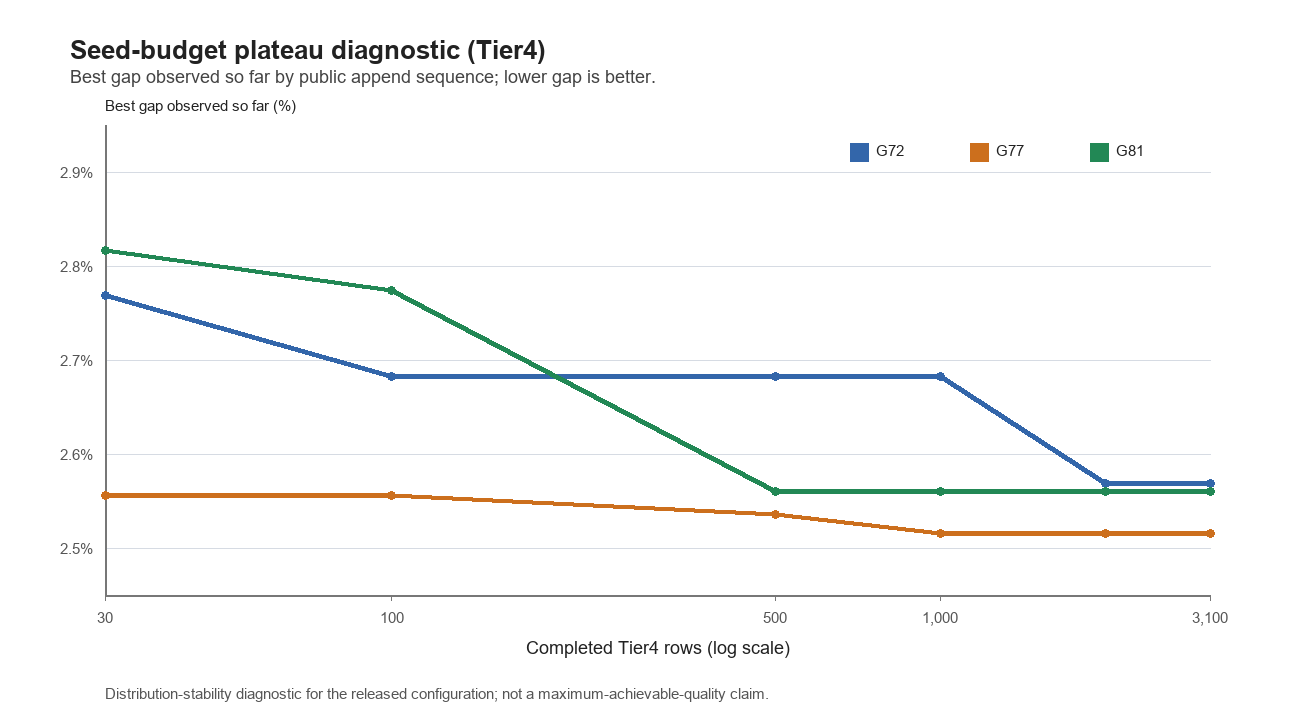
\includegraphics[width=0.90\linewidth]{figures/fig_seed_plateau_academic.png}
\caption{Seed-budget plateau diagnostic from the public Tier4 frontier extract. The plot starts at the equal-$N=30$ checkpoint and uses a log-scaled completed-row axis; it is a distribution-stability diagnostic, not a timing, matched-baseline, or maximum-achievable-quality claim.}
\label{fig:seedplateau}
\end{figure}

\clearpage

\subsection{Controlled Baseline Boundary}
The equal-$N$ controlled-baseline summary is deliberately treated as context rather than the center of the paper. It demonstrates how the source-lock protocol records a small external-reference check while preventing that check from becoming a stronger public claim than the artifacts support. Equal $N$ does not imply equal compute budget, and the best-of-$N$ summary does not meet the same distributional reporting standard as the public B1Brain frontier extract. The summary table is provided in Appendix~\ref{sec:controlledappendix}; raw controlled baseline rows, exact command pins, and distributional baseline traces are not part of the public package.

\subsection{Excluded Rows}
The parsed final frontier claim sets contain 3,006 Tier2, 3,501 Tier3, and 9,300 Tier4 completed rows, with zero non-claim rows and zero parse errors in those claim files. Status and capability-boundary records are preserved outside the performance denominator. This separation is central to the methodology: excluded rows remain auditable but do not support solver-performance claims.

\section{Threats to Validity and Limitations}
\paragraph{Construct validity.}
G72, G77, and G81 are evaluated against current best-known heuristic values, not proven optima. If future work proves those values optimal, the reported gaps can be reinterpreted against an optimum without changing the public rows. If future work improves those values, the source-lock registry and public CSVs allow the gaps to be recomputed. The impossible-result guard is therefore not expected to fire in the frontier lane; it applies to certified-value lanes such as BiqMac parity, where a reported value above the certified reference is treated as evidence of mapping or data-integrity error, not as a solver breakthrough.

\paragraph{Internal validity.}
The controlled baseline lane is summary-level and context-only. Exact command pins, seed lists, compile flags, stopping rules, tuning policy, hardware annotations, per-restart budgets, and raw controlled rows must be released or made available under controlled review before third parties should treat the MQLib/open SB comparison as independently rerunnable. The $N=30$ result is therefore not a public dominance, matched-compute, fairness, or rerunability claim. Asymmetric source-locking is the main release risk: the instance files are already pinned more completely than the comparison solver executions. This asymmetry does not invalidate the protocol contribution because all public claims are limited to what the released evidence supports; it limits the controlled baseline lane to context until the baseline execution artifacts are source-locked and released.

\paragraph{External validity.}
The frontier lane uses three structurally related Gset instances because they have clean source-locked current best-known values and a complete public per-run extract. G63, G64, Tabu Search/MaxCut-Bench-style baselines, broader Gset, BiqMac, grid-derived, finance, and other vertical comparisons are deferred or separated into non-frontier lanes until objective conventions, sources, implementations, command pins, and baselines are locked for each compared solver. One grid-derived comparison in earlier internal work favored open SB over B1Brain; it is excluded here because that lane is not source-locked, not because of the outcome. The paper does not claim global Gset leadership or broad vertical superiority.

\paragraph{Reproducibility boundary.}
The public package supports summary-level and redacted per-run objective verification. It does not provide full public rerunability of the proprietary solver, unredacted JSONL traces, timing logs, or solution bitstrings. Independently checkable bitstrings would strengthen external validation, but they remain a controlled-review artifact pending IP and disclosure review. Bitstrings may be released under controlled review after clearance; no public timeline is guaranteed.

\paragraph{Timing and resource use.}
The paper makes no claim about timing, throughput, time-to-target, GPU-hours, or energy use. Timing evidence requires dedicated, uncontended hosts and a separate release lane; otherwise it would conflate quality and resource consumption.

\section{Verification Protocol}
An independent reviewer can verify the central claims without solver internals:
\begin{enumerate}
  \item confirm public best-known values against cited sources;
  \item confirm that the benchmark instance names, objective conventions, cited best-known values, and value-type labels match the public source references, and recompute SHA-256 checksums for released CSVs and scripts from the public supplement manifest;
  \item inspect public redacted per-run rows, or controlled raw rows under review, and count only completed solver rows;
  \item check that non-claim rows are excluded from performance denominators;
  \item where access is granted, rerun bounded seed ranges through a documented external interface;
  \item compare new objectives against the reported tail distributions; and
  \item if bitstrings are later released, recompute cut values directly from pinned instance files.
\end{enumerate}

\section{Conclusion}
We presented a source-locked, append-only, tail-aware evaluation methodology for QUBO/Ising solvers and applied it to a proprietary black-box solver across heterogeneous local compute tiers. The evidence shows repeated local execution under audit discipline: 20,223 completed public-safe solver rows, stable distribution-level cross-tier behavior, explicit row-exclusion discipline, and a context-only controlled-baseline lane whose missing raw artifacts are not promoted into stronger claims. The main contribution is not an overclaim of solver supremacy, but a defensible framework for measuring black-box optimization systems under data-integrity and public-disclosure constraints. For practitioners evaluating a proprietary optimizer, the reusable lesson is the protocol: source-identify instances and baselines, checksum released artifacts, preserve non-claim rows, separate evidence lanes, publish distributional extracts, and keep timing, energy, baseline-rerunability, and leadership claims out of scope until those lanes are independently source-locked.

\clearpage
\appendix
\section{Public Validation Artifacts}
The public source package includes public-safe validation tables and a redacted ancillary supplement that support the figures and summary tables without exposing protected solver internals. The public evidence repository is available at \url{https://github.com/bernie-b1stAI/b1brain-qubo-ising-evaluation}. The supplement releases the complete 15,807-row redacted frontier extract for G72/G77/G81, plus per-run objective rows for locally mirrored Gset breadth and BiqMac parity lanes. The unredacted append-only JSONL records and solution bitstrings remain controlled-review artifacts until a separate public-release decision is made.

\begin{table}[tbp]
\centering
\caption{Public validation artifacts included in the source package.}
\label{tab:artifacts}
\footnotesize
\begin{tabular}{@{}L{0.46\linewidth}L{0.46\linewidth}@{}}
\toprule
File & Purpose \\
\midrule
\path{data/frontier_large_seed_summary.csv} & Claim-valid G72/G77/G81 frontier distributions by tier. \\
\path{data/controlled_maxcut_comparison.csv} & Context-only equal-$N=30$ B1Brain/open SB/MQLib summary values; raw baseline rows and commands are not public. \\
\path{data/hardware_evidence_matrix.csv} & Public-safe local hardware tier evidence matrix. \\
\path{data/exclusion_registry.csv} & Summary of exclusion categories and denominator rules. \\
\path{data/validation_manifest.csv} & Scope, public-release status, and reviewer-use notes for included and held-back artifacts. \\
\path{data/tier_invariance_diagnostics.csv} & Distribution-level cross-tier descriptive diagnostics computed from the public frontier extract. \\
\path{data/seed_plateau_summary.csv} & Tier4 seed-budget plateau checkpoints generated from the public frontier extract. \\
\path{figures/fig_evidence_volume_academic.png} & Claim-valid evidence volume visualization generated from public-safe lane counts. \\
\path{figures/fig_row_admissibility_flow_academic.png} & Visual row-admissibility pipeline and denominator boundary. \\
\path{figures/fig_gap_boxplot_academic.png} & Box summaries of public frontier gap distributions by instance and tier. \\
\path{figures/fig_gap_ecdf_academic.png} & ECDF visualization generated directly from the public frontier extract. \\
\path{figures/fig_seed_plateau_academic.png} & Best-gap-so-far plateau diagnostic generated directly from the public frontier extract. \\
\path{anc/b1brain_public_supplement_2026-05-31/README.md} & Public supplement guide, lane boundaries, and redaction policy. \\
\path{anc/b1brain_public_supplement_2026-05-31/evidence_lane_inventory.csv} & Lane inventory separating frontier, Gset breadth, BiqMac parity, controlled baselines, and hardware evidence. \\
\path{anc/b1brain_public_supplement_2026-05-31/frontier_per_run_public_extract.csv} & Complete 15,807-row redacted public frontier extract for G72/G77/G81. \\
\path{anc/b1brain_public_supplement_2026-05-31/gset_breadth_per_run_public.csv} & Redacted completed per-run Gset breadth rows; timing and implementation fields removed. \\
\path{anc/b1brain_public_supplement_2026-05-31/biqmac_parity_per_run_public.csv} & Redacted completed per-run source-repaired BiqMac parity rows. \\
\path{anc/b1brain_public_supplement_2026-05-31/verify_public_supplement.py} & Verifier for public row counts, lane inventory, redaction boundaries, and checksum manifest consistency. \\
\path{anc/b1brain_public_supplement_2026-05-31/reproduce_public_summaries.py} & Standard-library script that recomputes the public frontier summary table from released CSV rows. \\
\path{anc/b1brain_public_supplement_2026-05-31/checksum_manifest.csv} & SHA-256 manifest for public supplement artifacts. \\
\path{anc/b1brain_public_supplement_2026-05-31/schema.md} & Public field dictionary and redaction notes for released CSV artifacts. \\
\path{anc/b1brain_public_supplement_2026-05-31/bitstring_release_status.csv} & Explicit status marker explaining that solution bitstrings are not included in this public release. \\
\path{anc/b1brain_public_supplement_2026-05-31/deferred_release_gates.csv} & Public-safe checklist of artifacts required before stronger bitstring, baseline, Tabu, timing, or related-work claims. \\
\bottomrule
\end{tabular}
\end{table}

\begin{table}[tbp]
\centering
\caption{Deferred release gates for stronger future claims. These are not current claims; they define what must be added before a stronger statement is scientifically or legally safe. No target dates are stated; releases require separate legal, IP, and disclosure clearance.}
\label{tab:deferredgates}
\footnotesize
\begin{tabular}{@{}L{0.22\linewidth}L{0.35\linewidth}L{0.31\linewidth}@{}}
\toprule
Lane & Required public or controlled-review artifact & Current boundary \\
\midrule
Frontier bitstrings & One best-cut bitstring per G72/G77/G81 plus a verifier & Held pending IP and disclosure review; objectives are not public cut certificates. \\
Controlled baselines & Raw $N=30$ rows, command pins, seeds, versions, stopping rules, and build notes & Summary-only; not independently rerunnable from public files. \\
Tabu/MaxCut-Bench & Pinned public Tabu or BLS implementation, restart policy, stopping rule, and command transcript & Deferred context only; no Tabu comparison result is claimed. \\
G63/G64 extension & Source-locked references, row extracts, and baseline comparison artifacts & Outside the current G72/G77/G81 frontier claim lane. \\
Gset instance-file digests & Separate public SHA-256 manifest for raw Gset instance files & Current release records public source, instance name, objective convention, and cited value, but not independent instance-file hashes. \\
Timing/resource lane & Dedicated-host timing logs, resource traces, and time-to-target definitions & No speed, throughput, energy, or perf-per-watt claim. \\
Related-work and public-package sweep & Submission sweep completed on 2026-06-04; re-check if submission is delayed materially & Do not promote unverified secondary observations to citations. \\
\bottomrule
\end{tabular}
\end{table}

\section{Verifier Output and Exclusion Taxonomy}
The public supplement includes a local verifier. The expected successful run reports:
\begin{center}
\footnotesize
\begin{tabular}{lr}
\toprule
Check & Value \\
\midrule
Frontier public extract rows & 15,807 \\
Gset breadth public rows & 330 \\
BiqMac parity public rows & 90 \\
Inventory lanes & 6 \\
Redaction rules & 5 \\
Checksum manifest entries & 16 \\
Supplement SHA-256 & \texttt{736dd2...50b41} \\
Status & PASS \\
\bottomrule
\end{tabular}
\end{center}

The companion reproducer reports \path{frontier_large_seed_summary.csv}: PASS after recomputing the nine public frontier summary rows from the released 15,807-row extract. The supplement SHA above is an aggregate fingerprint over the public supplement. Table~\ref{tab:keychecksums} gives per-file CSV fingerprints; these are intentionally different integrity surfaces.

\begin{table}[tbp]
\centering
\caption{Selected CSV artifact SHA-256 prefixes.}
\label{tab:keychecksums}
\footnotesize
\begin{tabular}{@{}L{0.48\linewidth}L{0.30\linewidth}r@{}}
\toprule
File & SHA-256 prefix & Public rows \\
\midrule
\texttt{frontier\_per\_run\_public\_extract.csv} & \texttt{2959ad88038f} & 15,807 \\
\texttt{frontier\_large\_seed\_summary.csv} & \texttt{4ef6a6a933ce} & 9 \\
\texttt{controlled\_maxcut\_comparison.csv} & \texttt{76a1bd89c8e0} & 3 \\
\texttt{evidence\_lane\_inventory.csv} & \texttt{d680855f8983} & 6 \\
\texttt{exclusion\_registry.csv} & \texttt{adb4748dd5f0} & 8 \\
\bottomrule
\end{tabular}
\end{table}

\begin{table}[tbp]
\centering
\caption{Public exclusion taxonomy. Excluded categories are preserved for audit but never counted as completed solver-performance rows.}
\label{tab:exclusions}
\footnotesize
\begin{tabular}{@{}L{0.25\linewidth}L{0.34\linewidth}L{0.33\linewidth}@{}}
\toprule
Class & Rule & Claim implication \\
\midrule
Capability boundary & Count separately; never solver performance & Honesty evidence, not performance evidence \\
Investigation failure & Preserve for audit trail & Do not hide and do not count as completed \\
Runtime dependency missing & Environment failure, not solver quality & Infrastructure maturity only \\
Summary/status file & Not a solver row & Never count as completed rows \\
Stale status metadata & Supervisor said running while no queue existed & Treat as stale metadata \\
Superseded non-JAX Tier4 rows & Superseded by \texttt{\_jaxfixed} result files & Exclude from Tier4 performance claims \\
Contended Tier2 timings & Development laptop timing lane & Exclude from timing, throughput, and energy claims \\
Inferred formulations & Not first-hand verified from source & Do not run or cite external claims \\
\bottomrule
\end{tabular}
\end{table}

\clearpage

\section{Reviewer Reproducibility Checklist}
\begin{table}[H]
\centering
\caption{What an external reviewer can verify from the public package, and what remains controlled-review only.}
\label{tab:reviewchecklist}
\footnotesize
\begin{tabular}{@{}L{0.31\linewidth}L{0.22\linewidth}L{0.39\linewidth}@{}}
\toprule
Item & Public status & Notes \\
\midrule
Paper tables and row counts & Public & Recomputed from included CSVs and verifier output \\
G72/G77/G81 per-run objectives & Public redacted & Complete 15,807-row frontier extract \\
Gap formula and objective convention & Public & Defined in Appendix~\ref{sec:objectiveconvention} \\
Gset breadth and BiqMac parity rows & Public redacted & Separate breadth/parity lanes, not leadership claims \\
Controlled baseline raw rows & Controlled review & Needed before independent rerun claims \\
Baseline commands and exact versions & Controlled review/pending redaction & Required for full rerunability of Table~\ref{tab:controlled} \\
Solver executable or API & Controlled review & Black-box release boundary \\
Solution bitstrings & Controlled review & Strongest future artifact for independent cut validation \\
Timing logs and resource traces & Not claimed & Requires a separate dedicated timing lane \\
\bottomrule
\end{tabular}
\end{table}

\clearpage

\section{Context-Only Controlled Baseline Appendix}
\label{sec:controlledappendix}
The controlled-baseline summary is included to show how the protocol records external-reference context under an equal-$N$ restart-count quality summary without turning that context into a leaderboard claim. Equal $N$ matches restart count only; it does not normalize computational budget or per-restart work. Because the current public release exposes only summary values for the baseline lane, the table below should not be interpreted as independently rerunnable until raw controlled rows, exact command pins, seed lists, versions, stopping rules, MQLib heuristic selection, and open SB parameter policy are released or made available under controlled review. Because it is best-of-$N$ and not distributional for the baselines, this table is also not held out as satisfying the same distributional standard as the public B1Brain frontier extract.

\begin{table}[H]
\centering
\caption{Context-only controlled Max-Cut summary, best-of-$N$ gap to current best-known heuristic value. This table is not an independently rerunnable baseline claim; equal $N$ means equal restart count, not equal compute budget. Raw controlled baseline rows, exact baseline command pins, and distributional statistics are not public, so the ordering should not be read as a statistical significance, fairness, solver-superiority, or matched-compute claim.}
\label{tab:controlled}
\small
\begin{tabular}{lrrr}
\toprule
Instance & MQLib & B1Brain & Open SB implementation \\
\midrule
G72 & 2.08\% & 2.77\% & 3.05\% \\
G77 & 1.87\% & 2.66\% & 2.96\% \\
G81 & 1.96\% & 2.80\% & 3.24\% \\
\bottomrule
\end{tabular}
\end{table}

\clearpage

\section{Data Availability and Disclosure Boundary}
Public-safe validation artifacts are included in the public source package and ancillary supplement at \url{https://github.com/bernie-b1stAI/b1brain-qubo-ising-evaluation}. Unredacted JSONL rows, controlled baseline traces, exact solver-interface details, solution bitstrings, and timing logs are not part of the public package. They may be made available only under controlled review after IP, patent, export-control, and disclosure clearance; no release timeline is guaranteed for controlled artifacts. The author declares no external funding and no competing interests. The public source package has been cleared for submission under the stated disclosure boundary.

\section{Objective Convention}
\label{sec:objectiveconvention}
For Gset Max-Cut rows, the reported objective follows the standard higher-is-better cut-value convention:
\[
  \mathrm{cut}(x)=\sum_{(i,j)\in E} w_{ij}\mathbf{1}[x_i \ne x_j].
\]
The reported gap is
\[
  100 \times \frac{v_{\mathrm{best-known}} - v_{\mathrm{run}}}{v_{\mathrm{best-known}}},
\]
where $v_{\mathrm{best-known}}$ is a current best-known heuristic value, not a proven optimum, for G72, G77, and G81. Rows from certified-value datasets are handled separately through the impossible-result guard described in the methodology.

\section{Reproducibility Status}
The public package is reproducible at the summary level and at the redacted per-run objective level: a reader can inspect the CSVs, compare them with the printed tables and figures, run the public verifier, verify the lane inventory and checksums, and confirm that the paper's stated claims match the disclosed evidence. A stronger artifact would include unredacted raw JSONL rows under controlled review, per-run objective traces, and independently checkable solution bitstrings. Those artifacts would improve scientific reproducibility, but they also require a separate IP and disclosure review because this paper treats the solver as a proprietary black box. Until that release decision is made, the paper intentionally limits itself to quality, distributional robustness, source-locking, and exclusion-discipline claims.

\bibliographystyle{plainnat}
\bibliography{references}

\end{document}
